\tikzstyle{end} = [circle, minimum width = 4pt, fill, inner sep = 1pt,
	opacity = 1]
\tikzstyle{start} = [circle, inner sep = 1pt, opacity = 0]

\onslide<1->{
\tikzstyle{end3} = [circle, minimum width = 4pt, fill, inner sep = 1pt,
	opacity = 0]
%\tikzstyle{end5} = [circle, minimum width = 4pt, fill, inner sep = 1pt,
%	opacity = 0]
}

\only<3->{
	\tikzstyle{end3} = [circle, minimum width = 4pt, fill, inner sep = 1pt,
		opacity = 1]
}
%\only<5->{
	\tikzstyle{end5} = [color = red, circle, minimum width = 4pt, fill, inner sep = 1pt,
		opacity = 1]
%}
            
\tikzstyle{level 1} = [level distance = 0.1cm, sibling distance = 0.4cm]
\tikzstyle{level 2} = [level distance = 0.8cm]
\tikzstyle{level 3} = [level distance = 1cm]
\tikzstyle{level 4} = [level distance = 0.4cm]

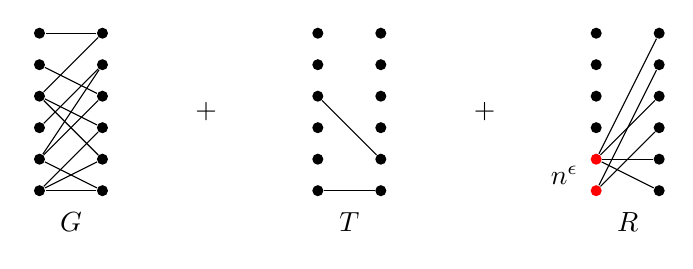
\begin{tikzpicture}[grow = right]
    \node [start]{}
    	child foreach \i in {6, ..., 1}{
            node [end] (x\i) {}
               	child [end]{
	             	node [end] (y\i){}
    	            edge from parent [opacity = 0]
        	    }
            edge from parent [opacity = 0]
        };

    \path [draw, opacity = 1](y1) -- (x3);
    \path [draw, opacity = 1](y1) -- (x1);
    \path [draw, opacity = 1](y2) -- (x4);
    \path [draw, opacity = 1](y2) -- (x5);
    \path [draw, opacity = 1](y3) -- (x5);
    \path [draw, opacity = 1](y3) -- (x2);
    \path [draw, opacity = 1](y4) -- (x3);
    \path [draw, opacity = 1](y4) -- (x6);
    \path [draw, opacity = 1](y5) -- (x3);
    \path [draw, opacity = 1](y5) -- (x6);
    \path [draw, opacity = 1](y6) -- (x5);
    \path [draw, opacity = 1](y6) -- (x6);

    \path [opacity = 0](y6) -- (x6) node [start, midway] (mid){};
    \node at (mid.south) [below = 0.1cm] {$G$};

    \path [opacity = 0](y3) -- (y4) node [start, midway] (mid2){};
    \node <.(2)-> at (mid2.east) [right = 1cm] (plus) {$+$};

    \node <.(3)-> at (plus.east) [right = 1cm, start]{}
    	child foreach \i in {6, ..., 1}{
            node [end3] (xx\i) {}
               	child [end3]{
	             	node [end3] (yy\i){}
    	            edge from parent [opacity = 0]
        	    }
            edge from parent [opacity = 0]
        };

    \path <.(3)-> [draw, opacity = 1](yy5) -- (xx3);
    \path <.(3)-> [draw, opacity = 1](yy6) -- (xx6);

    \path <.(3)-> [opacity = 0](yy6) -- (xx6) node [start, midway] (mid){};
    \node <.(3)-> at (mid.south) [below = 0.1cm] {$T$};

    \path <.(3)-> [opacity = 0](yy3) -- (yy4) node [start, midway] (mid3){};
    \node <.(4)-> at (mid3.east) [right = 1cm] (plus2) {$+$};

    \node <.(5)-> at (plus2.east) [right = 1cm, start]{}
    	child foreach \i in {6, 5}{
            node [end5] (xxx\i) {}
               	child [end]{
	             	node [end] (yyy\i){}
    	            edge from parent [opacity = 0]
        	    }
            edge from parent [opacity = 0]
        }
        child foreach \i in {4, ..., 1}{
            node [end] (xxx\i) {}
               	child [end]{
	             	node [end] (yyy\i){}
    	            edge from parent [opacity = 0]
        	    }
            edge from parent [opacity = 0]
        };

    \path <.(5)-> [draw, opacity = 1](xxx5) -- (yyy1);
    \path <.(5)-> [draw, opacity = 1](xxx6) -- (yyy2);
    \path <.(5)-> [draw, opacity = 1](xxx5) -- (yyy3);
    \path <.(5)-> [draw, opacity = 1](xxx6) -- (yyy4);
    \path <.(5)-> [draw, opacity = 1](xxx5) -- (yyy5);
    \path <.(5)-> [draw, opacity = 1](xxx5) -- (yyy6);

    \path <.(5)-> [opacity = 0](yyy6) -- (xxx6) node [start, midway] (mid3){};
    \node <.(5)-> at (mid3.south) [below = 0.1cm] {$R$};

    \path <.(5)-> [opacity = 0](xxx6) -- (xxx5) node [start, midway] (mid4){};
    \node <.(5)-> at (mid4.west) [left = 0.05cm] {$n^{\epsilon}$};
\end{tikzpicture}
